\section{Introduction}
La conception d'un appareil de palpation pour nodules pulmonaires est un projet entrepris conjointement par les services du BEAMS et du SAAS. L'objectif de ce dernier serait de remplacer les cours d'\textit{Instrumentation} et d'\textit{Automatique} actuellement donnés en BA3. Cela permettrait en effet aux futurs étudiants d'acquérir les mêmes compétences, mais de manière beaucoup plus didactique.\\

Dans le cadre du cours d'\textit{Active Medical Devices}, il a donc été demandé de collaborer à ce projet en développant une interface graphique. Celle-ci permettrait de faire le lien entre les étudiants et l'appareil de palpation, en affichant notamment les données mesurées par les différents capteurs sous forme de graphiques, en offrant la possibilité d'enregistrer ces résultats dans un fichier, etc.\\

Au cours de l'année passée, une première ébauche d'interface graphique avait été mise en place par Andréa Thibaud durant son stage. Il s'agissait en réalité d'un fichier Excel permettant de faire l'affichage des données envoyées depuis la carte Arduino. Cette solution n'étant pas optimale, il a été décidé après discussion avec le superviseur du projet de réaliser l'interface graphique grâce à Python.\\

Il est important de noter que ce rapport ne suit pas exactement la structure d'un rapport scientifique classique. Celui-ci a en effet été écrit avec l'intention de servir de guide afin de permettre aux futurs étudiants de comprendre le code informatique et le fonctionnement de l'interface graphique avec plus de facilité.\\

Le code Python est disponible à cette adresse: \url{https://github.com/thomasninane/didactic_palpation_device}.\\

Le code \LaTeX\ de ce document a été ajouté au projet GitHub afin que les explications concernant le code puissent être mises à jour en fonction de l'évolution du projet.\\

La section \ref{sec:explication_code} explique le code Python qui permet de créer l'interface graphique. Afin de permettre une compréhension maximale, il faut noter que chaque méthode a aussi été commentée directement dans le code.

\newpage
\section{Cahier des charges}

Afin de mieux visualiser les fonctionnalités devant être implémentées, un cahier des charges a été réalisé. Il est repris ci-dessous:

\begin{enumerate}
    \item Présence de commentaires dans le code afin d'en faciliter la compréhension.
    \item L'interface doit être intuitif et facile d'utilisation pour les étudiants qui s'en serviront durant les prochaines années.
    \item Les courbes à afficher sont: commande, position, vitesse et force.
    \item Les courbes doivent être affichées sur des graphiques différents.
    \item Un même graphique doit pouvoir afficher 2 courbes: celle de la partie maître et celle de la partie esclave (exemple: commande maître et commande esclave sur le graphique "commande").

     
    \item Explorer les limites de l'Arduino et de l'interface graphique concernant l'affichage et le rapatriement des données sur l'ordinateur. Idéalement, on voudrait acquérir les données toutes les millisecondes et actualiser l'interface toutes les 10 ou 100 millisecondes.
    
    \item Pour l'affichage en temps \textbf{non-réel}:
    \begin{enumerate}
        \item Présence d'un bouton \textit{SELECT FILE} permettant de choisir le fichier source (fichier \textit{.txt}).
        \item Implémentation d'une fonctionnalité permettant de générer les graphiques grâce à ce fichier source.
        \item Présence de boutons permettant d'afficher ou de cacher les courbes souhaitées (exemple: on veut parfois uniquement se concentrer sur la partie maître et cacher les courbes de la partie esclave).
    \end{enumerate}
    
    \item Pour l'affichage en temps \textbf{réel}:
    \begin{enumerate}
        \item Implémentation d'une fonctionnalité permettant d'acquérir de nouvelles données, de tracer les graphes en temps réel, de sauvegarder ces graphes et de sauvegarder les données acquises.
        \item Ces nouvelles données sont envoyées par l'Arduino.
        \item La communication entre l'Arduino et l'interface graphique doit se faire via un port série (port \textit{COM}).
        \item Implémentation de 3 cases d'input (valeur basse, valeur haute) afin de pouvoir appliquer un échelon sur la commande ainsi que la fréquence d'acquisition.
        \item Implémentation d'un bouton \textit{GO} qui enverrait les données des 3 cases d'input à l'Arduino, qui lancerait automatiquement l'acquisition par l'Arduino et l'affichage en temps réel des graphes.
        \item Présence d'un bouton \textit{STOP} qui envoie une instruction à l'Arduino lui demandant d'arrêter l'acquisition et l'envoi de nouvelles données.
        \item Présence d'un bouton \textit{EXPORT} permettant d'exporter les données acquises sous forme de fichier \textit{.txt}.
        \item Bouton \textit{RECALL} permettant de relancer l'acquisition après que celle-ci ait été arrêtée sans perdre les données acquises préalablement.
    \end{enumerate}
    
    \item Implémentation d'un message d'avertissement lorsqu'on clique sur la bouton "fermer le programme" indiquant à l'utilisateur que la fermeture de celui-ci entraîne la perte des acquisitions non sauvegardées.
    
    \item Fonctionnalités supplémentaires:
    \begin{enumerate}
        \item Superposition de courbes sur le même graphe (force et position par exemple).
        \item Convertir la commande en degrés
        \item Possibilité de faire un zoom sur les graphiques.
        \item Faire des vérifications avant d'envoyer les 3 valeurs des cases d'input (commande doit être entre 0 et 4095).
        \item Il est possible que les données doivent être sauvegardées sur le microcontrôleur et que celles-ci soient envoyées lorsque l'acquisition est arrêtée. Il faut donc s'assurer que l'interface arrive à gérer cette opération.
    \end{enumerate}
\end{enumerate}

\newpage
\section{Explication du code informatique}
\label{sec:explication_code}

Le code informatique contient 7 fichiers Python. Ils sont cités ci-dessous et leur rôle est détaillé dans les sous-sections ci-après.
\begin{enumerate}
    \item \textbf{main.py}
    \item \textbf{MainPage.py}
    \item \textbf{DrawPlotsParent.py}
    \item \textbf{DrawPlotsFromFile.py}
    \item \textbf{DrawPlotsRealTime.py}
    \item \textbf{DataOutputWindow.py}
    \item \textbf{GlobalConfig.py}
\end{enumerate}

\subsection{main.py}

Ce fichier crée la fenêtre principale grâce au module \textit{tkinter}. Elle contient donc la fonction \textit{main} ainsi qu'une classe: \textit{GUI}. Cette classe possède un attribut \textit{frames} qui est un dictionnaire. Celui-ci va contenir les différentes pages qui sont créées dans la fenêtre principale.\\

Le constructeur crée 3 pages: \textit{MainPage}, \textit{DrawPlotsRealTime} et \textit{DrawPlotsFromFile}. Cependant, lors du lancement de l'application, seule la page \textit{MainPage} est affichée. Il faut donc bien comprendre la différence entre les fenêtres et les pages.\\

On y voit aussi la présence de la méthode \textit{on\_closing()} qui permet d'avoir une fenêtre d'avertissement lorsque l'utilisateur désire fermer le programme.

\subsection{MainPage.py}

Cette classe constitue une page. Elle hérite donc de \textit{tkinter.Frame} et on y retrouve 3 éléments:
\begin{enumerate}
    \item Le nom de la page: "MAIN PAGE".
    \item Un bouton permettant d'accéder à la page "Draw Plots Real Time".
    \item Un bouton permettant d'accéder à la page "Draw Plots From File".\\
\end{enumerate}

\textbf{Note concernant le constructeur:} On y trouve un paramètre qui s'appelle \textit{controller}. Il s'agit de la classe "GUI" car celle-ci contient la méthode permettant de changer la page qui est affichée dans la fenêtre principale (pour rappel, 3 pages sont créées lors du lancement du programme mais elles ne sont jamais affichées simultanément).


\subsection{DrawPlotsParent.py}

Ce fichier est utile afin d'éviter de réécrire du code qui est commun à \textit{DrawPlotsRealTime} et \textit{DrawPlotsFromFile}. Il va donc permettre d'implémenter de l'héritage car les 2 pages citées précédemment se ressemblent fortement. \textit{DrawPlotsRealTime} et \textit{DrawPlotsFromFile} héritent des attributs et méthodes de \textit{DrawPlotsParent}.\\

Avant de détailler le contenu de ce fichier, il est important d'acquérir certains concepts de base du module \textit{tkinter}. Ce module permet de générer des interfaces graphiques et est doté des éléments suivants:

\begin{enumerate}
    \item \textbf{LabelFrame:} permet de créer un cadre vide. Ce cadre peut contenir un nom ou ne pas être nommé et ses bords peuvent être rendus invisibles. L'utilisation de cadres permet de faciliter le placement des différents éléments au sein d'une même page.
    
    \item \textbf{Button:} permet de créer un bouton, de lui donner un nom et de lier ce bouton à une commande/action.
    
    \item \textbf{Entry:} permet de créer un champ de texte afin de récupérer des informations entrées par l'utilisateur.
    
    \item \textbf{CheckButton:} permet de créer une boite à cocher. Ce \textit{CheckButton} doit être lié à une variable de type \textit{IntVar()} qui vaut 0 ou 1 selon que la case soit cochée ou non. Lorsqu'il est coché ou décoché, il est possible d'exécuter une action.
    
    \item \textbf{Label:} permet de créer une ligne de texte qui peut être affichée sur l'interface.\\
\end{enumerate}

Une fois l'élément créé, il faut ensuite l'afficher. Ceci peut se faire grâce à la méthode \textit{pack()} ou \textit{grid(row, column)}. Il est important de noter que ces deux méthodes ne peuvent pas être utilisées simultanément au sein d'un même \textit{LabelFrame}. La première méthode va simplement placer les éléments l'un en-dessous de l'autre, alors que la seconde permet de déterminer plus précisément l'endroit où l'on désire rajouter l'élément.

\subsubsection{Méthodes statiques}

Les méthodes statiques sont celles qui ne nécessitent pas l'existence d'un objet pour être exécutées. En python, cela revient à ne jamais avoir besoin d'un élément (attribut ou méthode) commençant par "self." car ce mot clé est équivalent à "this." en Java (voir cours INFO-H2001). Ce fichier contient 2 méthodes statiques:
\begin{enumerate}
    \item \textbf{convert\_position\_to\_degrees:} la position envoyée par l'Arduino peut être convertie en degrés grâce à cette fonction afin de mieux visualiser à quoi cette mesure correspond.
    \item \textbf{convert\_command\_to\_amps:} la commande envoyée par l'Arduino est une valeur comprise entre 0 (correspondant à -2A) et 4095 (correspondant à 2A). Si l'étudiant le désire, il peut afficher la commande en ampères grâce à cette fonction.
\end{enumerate}

\subsubsection{Constructeur}

Le constructeur contient tous les éléments communs aux deux pages qui sont utilisés afin d'afficher les graphes en temps réel ou non. Ces éléments sont détaillés ci-dessous:

\begin{enumerate}
    \item \textbf{Upper Frame:} ce cadre est utile afin d'afficher le titre de la page et d'avoir un bouton "retour" qui permet de retourner à la page principale.
    \item \textbf{Main Frame:} ce cadre est l'élément principal de la page. Il contient 2 éléments: un grand cadre (\textit{Figure Frame}) qui lui-même contient une figure à 4 graphes (4 "subplots") et le cadre de droite (\textit{Right Side Frame}).
    \item \textbf{Right Side Frame:} ce cadre se situe à droite des graphiques. Il contient toutes les options qui permettent d'interagir avec les graphes et de manipuler les données. On y retrouve plusieurs sous-cadres:
    \begin{enumerate}
        \item \textbf{Window Specific Frame:} c'est ce cadre qui va contenir les options qui ne sont pas communes entre \textit{DrawPlotsRealTime} et \textit{DrawPlotsFromFile}.
        \item \textbf{Output Window Button:} permet de créer une nouvelle fenêtre afin d'afficher les données contenues dans le fichier texte ou celles qui ont été acquises grâce à l'Arduino.
        \item \textbf{Plots Options Frame:} ce cadre va contenir 4 sous-cadres. Chaque sous-cadre contient les options spécifiques de la courbe à laquelle il se rapporte (vitesse, position, commande et force). Par exemple, pour la courbe de la commande, on a 3 options: afficher la commande en ampères, afficher les données de la partie maître et afficher les données de la partie esclave.\\
    \end{enumerate}
\end{enumerate}

Voici, ci-dessous, un schéma pouvant être utile à la visualisation des différents éléments de la page et à leur positionnement sur l'interface graphique:

\begin{center}
    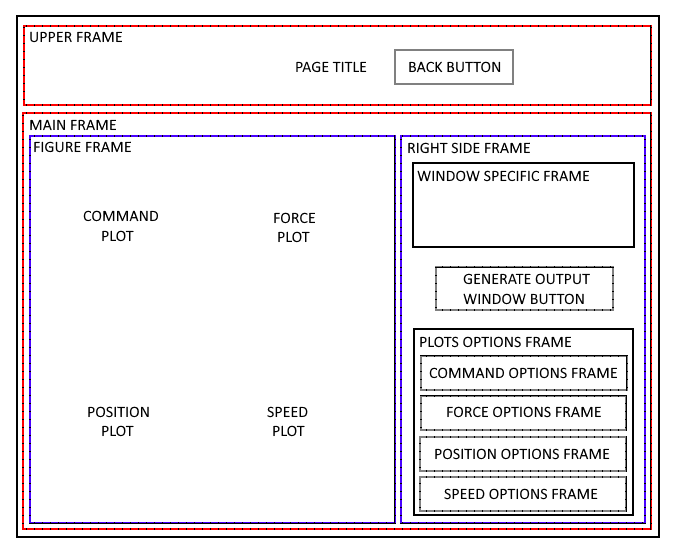
\includegraphics[width=15cm]{images/DrawPlotsParent-schematic.png}
    \captionof{figure}{Schéma de la page \textit{DrawPlotsParent}}
    \label{fig:schemaDrawPlotsParent}
\end{center}

Il faut aussi noter qu'il est de bonne pratique d'initialiser tous les attributs dans le constructeur. Ceux-ci doivent donc être initialisés à \textit{None}. Les 2 figures ci-dessous aident à comprendre cette procédure:

\begin{center}
    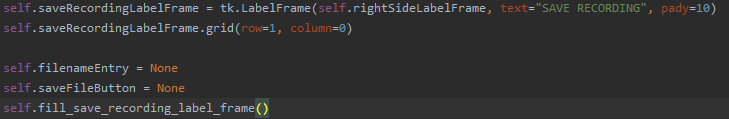
\includegraphics[width=15cm]{images/code1.png}
    \captionof{figure}{Code dans le constructeur}
    
    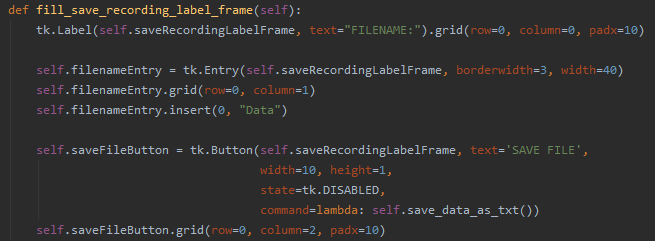
\includegraphics[width=15cm]{images/code2.png}
    \captionof{figure}{Méthode attribuant des objets aux attributs initialisés à "None" dans le constructeur. Le contenu de cette méthode n'est pas écrit dans le constructeur afin d'en alléger l'écriture.}
\end{center}


\subsubsection{Méthodes}

On distingue 2 catégories de méthodes: celles qui servent à ajouter des éléments graphiques dans les cadres (boutons, cases à cocher, etc.) et celles qui permettent d'effectuer des tâches ou des actions lorsque l'utilisateur clique sur un élément de l'interface.\\

Les méthodes appartenant à la première catégorie sont utiles afin d'alléger le constructeur et de compartimenter les différentes étapes réalisées lors de la création des pages \textit{DrawPlotsRealTime} et \textit{DrawPlotsFromFile}. Toutes les méthodes présentes dans \textit{DrawPlotsParent} sont reprises ci-dessous:

\begin{enumerate}
    
    \item \textbf{fill\_upper\_frame:} Remplit \textit{Upper Frame} avec le titre de la page et le bouton "retour" permettant de retourner au menu principal.
    
    \item \textbf{fill\_figure\_frame:} Remplit \textit{Figure Frame} avec une figure contenant 4 graphiques. Ce cadre est positionné à gauche et au centre de \textit{Main Frame}.\\
    On y trouve les méthodes \textit{FigureCanvasTkAgg()}, \textit{get\_tk\_widget()} et \textit{draw()} qui sont des méthodes spécifiques à l'affichage de figures dans une interface graphique avec le module \textit{tkinter}.
    
    \item \textbf{fill\_plots\_options\_frame:} Remplit \textit{Plots Options Frame}. On y retrouve une boucle qui va générer un cadre pour chaque type de graphique (commande, force, position et vitesse). Cette méthode réalise les opérations suivantes:
    \begin{enumerate}
        \item Création d'une zone de texte afin de donner un nom aux graphiques lors de leur sauvegarde sur le disque dur de l'ordinateur.
        \item Création d'un bouton engendrant la sauvegarde du graphique. Ce bouton est donc lié à la commande \textit{self.save\_plot()}. Lors de l'assignation de cette commande, on observe la méthode \textit{partial(function, function\_parameters)}. \textbf{Elle permet d'éviter un bug de l'interface lié à la boucle "for". Il faut donc éviter de modifier cette ligne}.
        \item Création des cases à cocher en appelant la méthode \textit{create\_check\_button()}. Celles-ci dépendent du type de graphe ce qui explique les nombreuses conditions "if". Par exemple, il n'y a pas de force pour la partie maître et il ne faut donc pas créer de case, il faut créer une case supplémentaire pour la commande afin de la convertir en ampères, etc.
    \end{enumerate}
    
    \item \textbf{create\_check\_button:} Cette méthode crée une case à cocher. La case qui est créée est liée à la commande \textit{refresh\_all\_plots()} si l'affichage n'est pas en temps réel. Cette commande va actualiser les graphes afin d'afficher ce que l'utilisateur désire (par exemple, si la case convertissant la commande en ampères est cochée, il faut que le graphique de la commande soit actualisé pour prendre en compte ce changement). A l'inverse, si l'affichage est en temps réel, il ne faut pas lier la case à une commande car les graphiques sont rafraîchis automatiquement.
    
    \item \textbf{clear\_all\_plots:} permet d'effacer toutes les courbes affichées sur les graphiques en conservant les noms des axes et les titres.
    
    \item \textbf{refresh\_all\_plots:} méthode qui est redéfinie dans les classes filles mais qui doit être définie dans la classe mère afin d'éviter une erreur de type "method out of scope".
    
    \item \textbf{activate\_or\_deactivate\_save\_plot\_buttons:} permet d'activer ou de désactiver tous les boutons liés à la sauvegarde des graphiques.
    
    \item \textbf{generate\_data\_output\_window:} crée une nouvelle fenêtre qui affiche les données acquises via l'Arduino ou celles du fichier texte.
    
    \item \textbf{destroy\_data\_output\_window:} ferme la fenêtre qui affiche les données. Cette fonction est utile lorsqu'un nouveau fichier texte est sélectionné ou qu'une nouvelle acquisition est démarrée.
    
    
    \item \textbf{add\_date\_to\_save\_name\_entries:} lorsque l'utilisateur désire sauvegarder des données sur le disque dur de l'ordinateur, il est important de rajouter la date et l'heure afin d'éviter que ces nouvelles données écrasent des fichiers déjà enregistrés préalablement. Cette opération est réalisée grâce à cette méthode.
    
    \item \textbf{save\_plot:} cette fonction permet de démarrer la sauvegarde d'un graphique. Elle appelle une des deux méthodes ci-dessous.
    
    \item \textbf{save\_plot\_normal\_axis:} permet la sauvegarde d'un graphe tout en respectant le choix de l'utilisateur d'afficher ou de cacher une des courbes (maître ou esclave).
    
    \item \textbf{save\_plot\_special\_axis:} permet la sauvegarde de la commande en ampères ou de la position en degrés tout en respectant le choix de l'utilisateur d'afficher ou de cacher une des courbes (maître ou esclave).
\end{enumerate}

\subsection{DrawPlotsFromFile.py}

Ce fichier permet de tracer les graphes à partir d'un fichier texte. Il hérite des méthodes et attributs de la classe \textit{DrawPlotsParent}. Ce choix permet de fortement simplifier le constructeur de cette classe ainsi que les méthodes qui doivent y être écrites.

\subsubsection{Méthodes statiques}

Ce fichier contient une seule méthode statique: \textit{create\_data\_frame()}. Lorsqu'un fichier texte est sélectionné, il faut rajouter les données qu'il contient à un \textit{data frame} (df) car c'est celui-ci qui est utilisé pour tracer et sauvegarder les courbes.

\subsubsection{Constructeur}

Le constructeur appelle la méthode \textit{super().\_\_init\_\_()} qui permet l'utilisation du constructeur de la classe mère. Il faut ensuite remplir \textit{Window Specific Frame} des éléments graphiques qui sont spécifiques à la classe fille.\\

Le seul bouton qui doit être rajouté est un bouton permettant de sélectionner un fichier texte sur le disque dur de l'ordinateur. Afin d'éviter toute ambiguïté, lorsqu'un fichier est sélectionné, il est important d'afficher son nom. Ce bouton et le nom du fichier sont rajoutés à \textit{File Selection Frame} qui lui-même est ajouté à \textit{Window Specific Frame}.

\begin{center}
    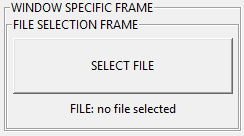
\includegraphics[scale=0.7]{images/DrawPlotsFromFile-WindowSpecificFrame.png}
    \captionof{figure}{DrawPlotsFromFile - WindowSpecificFrame}
\end{center}

\subsubsection{Méthodes}

Cette classe utilise 3 méthodes qui lui sont spécifiques:

\begin{enumerate}
    \item \textbf{fill\_file\_selection\_frame:} remplit \textit{File Selection Frame} afin d'alléger le constructeur.
    
    \item \textbf{import\_recording:} permet d'importer un fichier texte. Lorsque le fichier est sélectionné, le \textit{data frame} va être créé grâce à la méthode statique \textit{create\_data\_frame()} et utilisé afin d'afficher les courbes sur les 4 graphiques.
    
    \item \textbf{refresh\_all\_plots:} permet de rafraîchir les graphiques en prenant en compte les options cochées par l'utilisateur. Lorsque les graphiques ont été actualisés, la méthode va activer les boutons permettant leur sauvegarde. Cette méthode est appelée dès qu'un fichier texte a été choisi ou dès que l'état d'une case à cocher est modifié.
\end{enumerate}

\subsubsection{Capture d'écran}

La figure ci-dessous montre à quoi ressemble la page \textit{DrawPlotsFromFile} (note: afin de désengorger l'interface graphique, les bords et les noms de certains cadres ont été rendus invisibles).

\begin{center}
    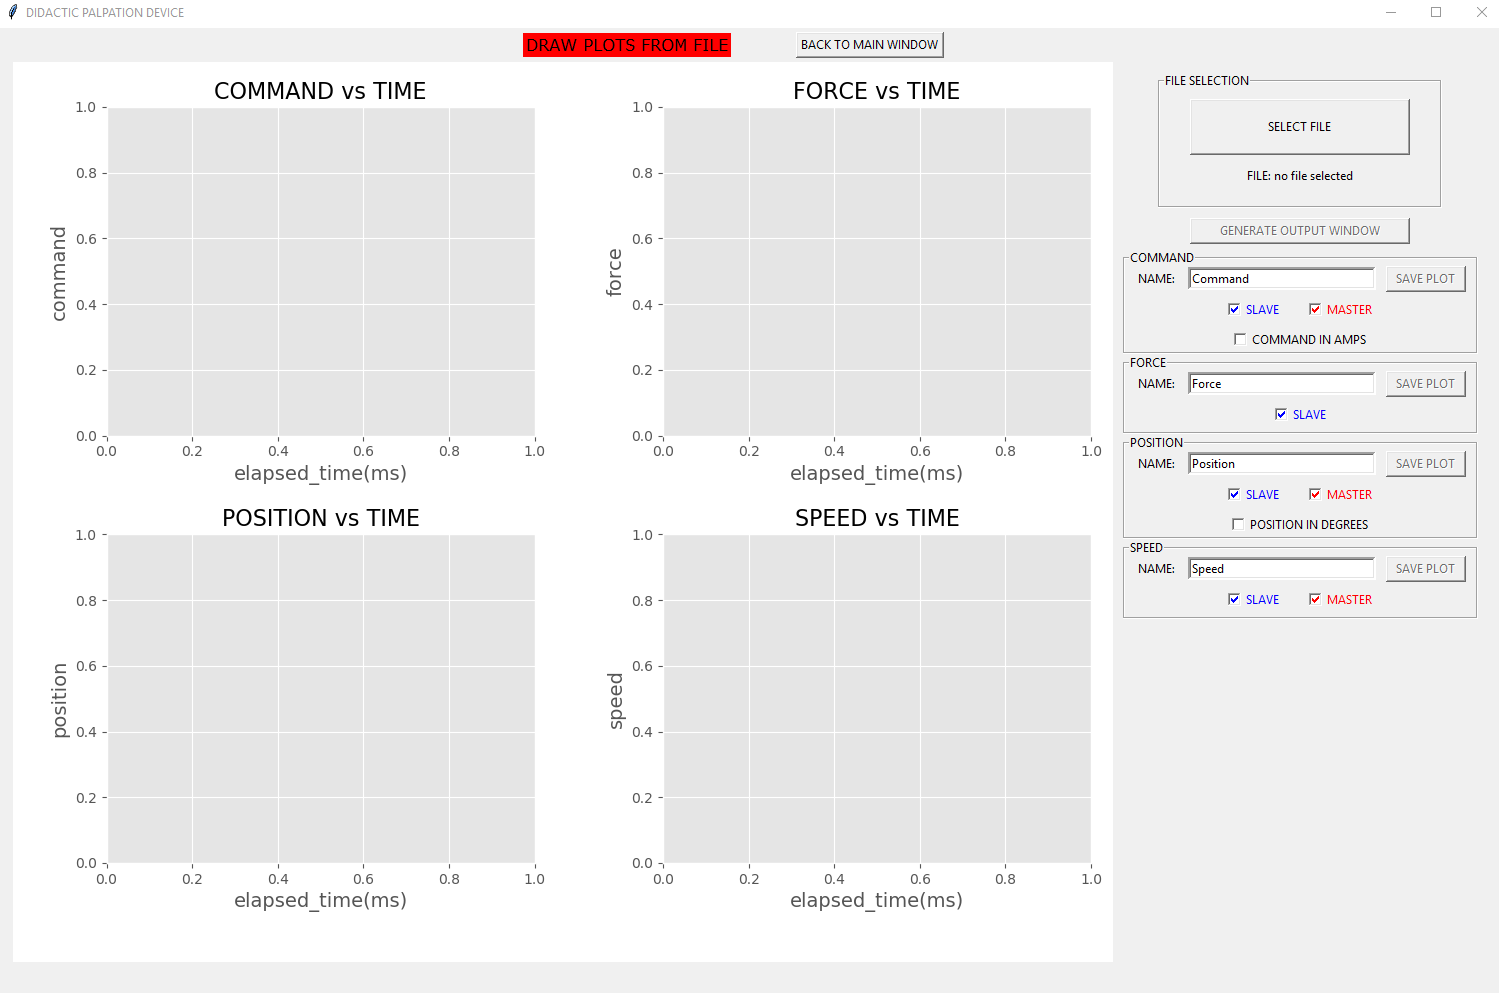
\includegraphics[width=16cm]{images/DrawPlotsFromFile-screenshot.png}
    \captionof{figure}{Capture d'écran: DrawPlotsFromFile}
\end{center}


\subsection{DrawPlotsRealTime.py}

Ce fichier permet de tracer les graphes à partir des données qui sont envoyées par l'Arduino. Il permet aussi de sauvegarder toutes les données reçues sous forme de fichier texte. Tout comme \textit{DrawPlotsFromFile}, cette classe hérite des attributs et des méthodes de \textit{DrawPlotsParent}.\\

Cette fenêtre peut fonctionner de 2 manières:
\begin{enumerate}
    \item Si un Arduino est connecté à l'ordinateur, celui-ci envoie les données au programme et l'interface les affiche sur les graphes en temps réel.
    \item Dans le cas où un Arduino n'est pas connecté, il est quand même possible de simuler une acquisition de données en temps réel. Ceci peut-être utile si l'utilisateur n'a pas accès au microcontrôleur mais qu'il désire quand même expérimenter avec l'interface graphique.\\
\end{enumerate}

\textbf{Note concernant le microcontrôleur:} Il ne faut pas oublier de modifier le paramètre \textit{COMMUNICATION\_PORT} qui se situe dans le fichier \textit{GlobalConfig}. De plus, l'Arduino doit être connecté à l'ordinateur avant le lancement du programme.

\subsubsection{Méthodes statiques}

Ce fichier contient une seule méthode statique: \textit{load\_simulation\_file()} qui est utile afin de simuler une acquisition de données. Elle charge un fichier texte qui à la même structure que lorsque c'est le microcontrôleur qui envoie les données. Ces données vont ensuite être utilisées par la méthode \textit{simulate\_real\_time\_data\_acquisition()}. Le fichier qui est utilisé pour cette simulation est défini par \textit{SIMULATE\_DATA\_ACQUISITION\_FILE} qui se situe dans \textit{GlobalConfig}.

\subsubsection{Constructeur}

Tout comme pour \textit{DrawPlotsFromFile}, le constructeur appelle la méthode \textit{super().\_\_init\_\_()} et il faut ensuite remplir \textit{Window Specific Frame} avec les éléments qui sont spécifiques à \textit{DrawPlotsRealTime}. Ceux-ci sont décrits ci-dessous:

\begin{enumerate}
    \item Un menu déroulant permettant de choisir si l'acquisition se fait grâce à un Arduino ou si elle est simulée à partir d'un fichier texte pré-existant (note: si le microcontrôleur n'est pas connecté ou que le port COM est mal configuré, seule l'option "simulation" est visible).
    \item \textbf{Acquisition Parameters Frame:} ce cadre contient tous les éléments qui sont nécessaires au lancement d'une nouvelle acquisition par le microcontrôleur.
    \item \textbf{Save Recording Frame:} ce cadre contient tous les éléments qui sont nécessaires à la sauvegarde des données reçues sous forme de fichier texte.
    \item \textbf{Refresh Plots Button:} lorsque l'acquisition est finie, le rafraîchissement des graphes ne se fait plus automatiquement. Par conséquent, si l'utilisateur désire modifier l'affichage (cacher une courbe ou alors modifier les unités pour la commande ou la position), il faut rafraîchir manuellement les graphes.
\end{enumerate}

\begin{center}
    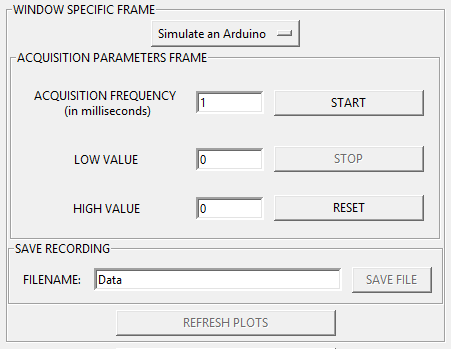
\includegraphics[scale=0.7]{images/DrawPlotsRealTime-WindowSpecificFrame.png}
    \captionof{figure}{DrawPlotsRealTime - WindowSpecificFrame}
\end{center}

\subsubsection{Méthodes}

Les méthodes utilisées par cette classe sont reprises ci-dessous:

\begin{enumerate}
    \item \textbf{fill\_acquisition\_parametersl\_frame:} remplit \textit{Acquisition Parameters Frame}. On y retrouve les éléments suivants:
    \begin{enumerate}
        \item L'intervalle (en millisecondes) entre 2 mesures acquises via l'Arduino.
        \item La valeur basse de la commande.
        \item La valeur haute de la commande.
        \item Un bouton "start" qui appelle la méthode \textit{start\_recording()}.
        \item Un bouton "stop" qui appelle la méthode \textit{stop\_recording()}.
        \item Un bouton "reset" qui appelle la méthode \textit{reset\_recording()}.
    \end{enumerate}
    
    \item \textbf{fill\_save\_recording\_frame:} remplit \textit{Save Recording Frame}. Permet d'enregistrer les données acquises sous forme de fichier texte tout en nommant ce fichier selon les désirs de l'utilisateur.
    
    \item \textbf{start\_recording:} cette méthode peut soit transmettre les valeurs utiles à l'Arduino (intervalle d'acquisition, valeur basse et valeur haute de la commande) et lui ordonner de commencer l'acquisition, soit charger un fichier qui va être utilisé afin de simuler une acquisition de données sans microcontrôleur via l'initialisation d'un Thread.
    
    \item \textbf{stop\_recording:} si l'acquisition se fait grâce au microcontrôleur, celui-ci reçoit une commande d'arrêt. Sinon, le Thread qui simule l'arrivée périodique de données est arrêté. De plus, le rafraîchissement automatique des graphes est interrompu.
    
    \item \textbf{reset\_recording:} cette méthode est utile afin de permettre une nouvelle acquisition en supprimant les données reçues, en effaçant les courbes sur les graphes et en activant ou désactivant certains boutons.
    
    \item \textbf{save\_data\_as\_txt:} permet de sauvegarder les données reçues sur le disque dur de l'ordinateur.
    
    \item \textbf{get\_acquisition\_parameters:} permet de récupérer les paramètres d'acquisition qui ont été entrés par l'utilisateur. Cette méthode vérifie que ces valeurs sont correctes et, le cas échéant, donne un message d'erreur.
    
    \item \textbf{send\_acquisition\_parameters\_to\_arduino:} envoie les paramètres d'acquisition vers le microcontrôleur. Voici un exemple d'envoi: "c10-1000-3000-1".
    \begin{enumerate}
        \item La lettre "c" est utile afin de signifier qu'un ordre est envoyé (commande). Toute information qui est envoyée vers l'Arduino et qui ne commence pas par la lettre "c" est ignorée.
        
        \item 10 représente la fréquence d'acquisition.
        
        \item 1000 représente la valeur basse de la commande.
        
        \item 3000 représente la valeur haute de la commande.
        
        \item 1 ordonne au microcontrôleur de démarrer l'acquisition.
    \end{enumerate}
    
    \item \textbf{simulate\_real\_time\_data\_acquisition:} les données chargées par \textit{load\_simulation\_file()} sont stockées dans \textit{self.simulation\_data}. Cette méthode tourne dans un Thread et va copier une ligne de \textit{self.simulation\_data} (la ligne dont l'index correspond à \textit{self.simulation\_step}) pour ajouter les valeurs aux listes qui contiennent les données acquises.
    
    \item \textbf{real\_time\_data\_acquisition:} cette méthode permet l'acquisition des données provenant de l'Arduino. Elle contient une boucle qui est exécutée tant que l'acquisition est en cours. On commence par lire le port série et séparer les différentes données envoyées (les valeurs envoyées vers l'ordinateur sont séparées par le caractère ";"). On rajoute ensuite les données à la liste adéquate (afin de mieux comprendre les opérations, il est utile de lire la section \ref{sec:remarque_acquisition}).
    
    \item \textbf{create\_data\_frame:} permet de créer un \textit{data frame} à  partir des données acquises via l'Arduino. Ce \textit{data frame} est ensuite utilisé pour sauvegarder les graphiques et pour sauvegarder ces données sous forme de fichier texte.
    
    \item \textbf{refresh\_all\_plots:} permet de rafraîchir les graphiques en prenant en compte les options cochées par l'utilisateur. Lorsque l'acquisition est terminée, la méthode va activer les boutons permettant leur sauvegarde. Cette méthode est appelée dès que l'utilisateur appuie sur le bouton \textit{Start} et est ensuite exécutée automatiquement toutes les 100 millisecondes (voir \textit{PLOTTING\_FREQUENCY} dans \textit{GlobalConfig}).
\end{enumerate}

\subsubsection{Capture d'écran}

La figure ci-dessous montre à quoi ressemble la page \textit{DrawPlotsRealTime} (note: afin de désengorger l'interface graphique, les bords et les noms de certains cadres ont été rendus invisibles).

\begin{center}
    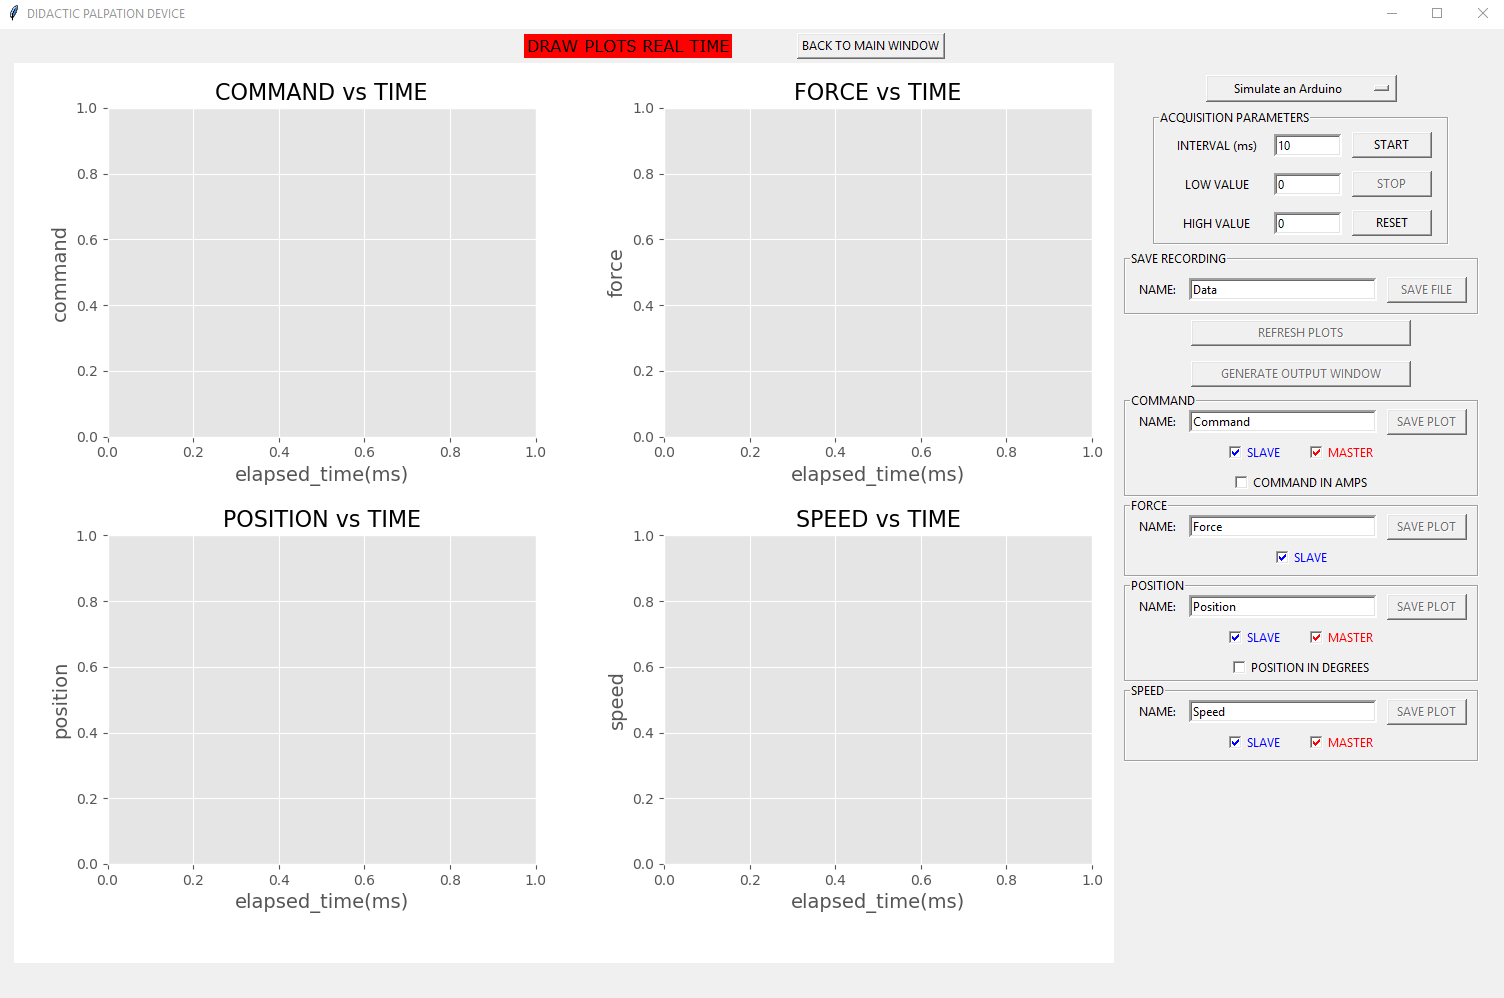
\includegraphics[width=16cm]{images/DrawPlotsRealTime-screenshot.png}
    \captionof{figure}{Capture d'écran: DrawPlotsRealTime}
\end{center}

\subsubsection{Remarque concernant l'acquisition en temps réel}
\label{sec:remarque_acquisition}

Lors de l'affichage des graphiques via le fichier texte, les données sont directement ajoutées à un \textit{data frame} car l'utilisation de celui-ci facilite la manipulation des colonnes (et donc l'affichage des graphiques ainsi que la sauvegarde de ceux-ci).\\

Cependant, lors de l'acquisition en temps réel, les données arrivent extrêmement rapidement et l'ajout d'une ligne à un \textit{data frame} existant n'est pas efficace du tout car cette méthode nécessite de copier l'entièreté du \textit{data frame} (l'opération prend parfois plusieurs millisecondes). Ceci provoque l'accumulation des données dans le \textit{buffer} du microcontrôleur, ce qui à 2 conséquences critiques. La première est que les données affichées par le programme ne sont plus des données en temps réel et la seconde est que lorsque ce \textit{buffer} est plein, il est automatiquement vidé ce qui provoque une perte énorme de données (à peu près 2 secondes de données sont perdues toutes les 6 secondes pour une fréquence d'acquisition de 10 millisecondes).\\

Afin de palier à ce problème, la procédure suivante est utilisée: un dictionnaire est créé et celui-ci contient 15 listes qui sont initialement vides. Les clés de ce dictionnaire sont les noms des colonnes (voir \textit{DATA\_FRAME\_COLUMNS} dans \textit{GlobalConfig}). Lorsqu'une nouvelle ligne de données est envoyée vers le programme, chaque élément est ajouté à la liste à laquelle il correspond car l'ajout d'un élément à une liste est extrêmement rapide.\\

Cette procédure implique 2 changements: 
\begin{enumerate}
    \item La méthode \textit{refresh\_all\_plots()} doit utiliser les listes du dictionnaire plutôt que les colonnes du \textit{data frame} afin d'afficher les graphiques en temps réel (voir les différences entre la méthode de \textit{DrawPlotsFromFile} et celle de \textit{DrawPlotsRealTime}).
    
    \item Une fois l'acquisition de données terminée, il est nécessaire de rajouter toutes les colonnes du dictionnaire à un \textit{data frame} afin de permettre la sauvegarde des graphiques et des données sur l'ordinateur.
\end{enumerate}

\subsection{DataOutputWindow.py}

Cette classe constitue une nouvelle fenêtre qui est appelée lorsque l'utilisateur clique sur le bouton \textit{Generate Output Window}. Elle permet d'afficher les données acquises via l'Arduino ou alors celles qui se situent dans un fichier texte.\\

Afin d'accéder aux attributs nécessaires à l'affichage des données, il faut avoir accès à \textit{DrawPlotsParent}. Ceci se fait grâce au paramètre \textit{parent} qui se situe dans le constructeur.\\

Comme l'entièreté des données ne peut être affichée sur l'écran (dans la direction horizontale), une barre de défilement horizontale a été rajoutée. De plus, si les données proviennent d'un fichier texte, le nom de ce fichier est affiché en haut de la fenêtre.

\subsection{GlobalConfig.py}

Ce fichier est utile afin de définir certains paramètres du programme sans devoir explorer l'ensemble des différents fichiers du projet. Voici quelques paramètres qui y sont définit:
\begin{enumerate}
    \item \textbf{APP\_GEOMETRY:} définit la dimension de la fenêtre principale.
    
    \item \textbf{OUPUT\_WINDOW\_GEOMETRY:} définit la dimension de la fenêtre qui affiche les données acquises via l'Arduino ou celles contenues dans un fichier texte. 
    
    \item \textbf{FIGURE\_X et FIGURE\_Y:} les dimensions de la figure qui contient les 4 graphes.
    
    \item \textbf{COMMUNICATION\_PORT:} le port \textit{COM} qui est en contact avec l'Arduino. Cette information peut être trouvée en allant dans le gestionnaire de périphériques (voir figure \ref{fig:port_com} ci-dessous).
    
    \item \textbf{BAUDRATE:} La vitesse de transmission des données entre l'Arduino et l'ordinateur. Cette valeur doit être identique dans le code Python et le code Arduino.
    
    \item \textbf{SIMULATE\_DATA\_ACQUISITION\_FILE:} il est possible de simuler une acquisition en temps réel sans Arduino. Celle-ci se fait à partir d'un fichier texte pré-existant et son chemin est défini ici.
    
    \item \textbf{SIMULATE\_DATA\_ACQUISITION\_INTERVAL:} l'intervalle entre l'ajout de 2 lignes de données lorsque l'acquisition en temps réel est simulée via un fichier texte.
    
    \item \textbf{PLOTTING\_FREQUENCY:} l'intervalle entre 2 actualisations des graphiques lors de l'affichage en temps réel (en millisecondes).
    
    \item \textbf{DATA\_FRAME\_COLUMNS:} les noms des grandeurs qui sont envoyées par l'Arduino. Il faut faire attention car une modification de cet élément a des conséquences sur l'ensemble du code Python et Arduino.
    
    \item \textbf{PLOT\_TYPES:} les noms des 4 types de graphes: commande, force, position et vitesse.
\end{enumerate}

\begin{center}
    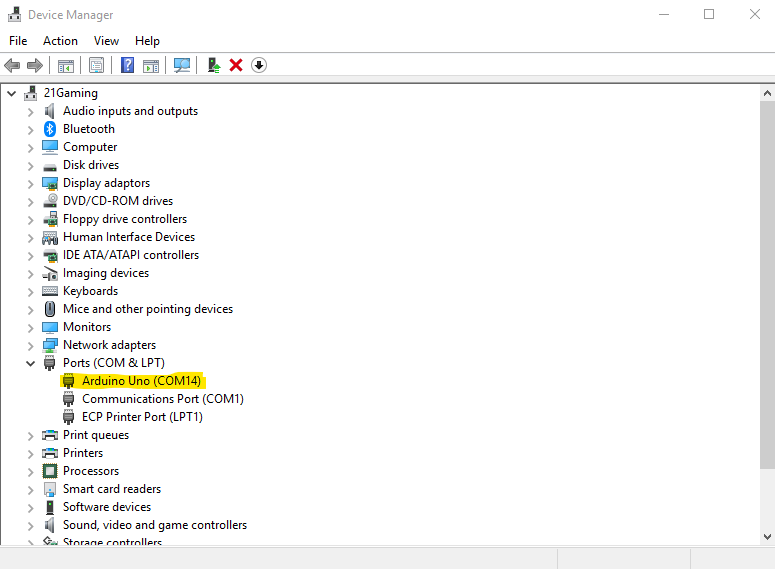
\includegraphics[scale=0.45]{images/device_manager.png}
    \captionof{figure}{Port COM}
    \label{fig:port_com}
\end{center}

\newpage
\section{Modifications du code de l'Arduino}

Comme nous n'avons pas accès au code Arduino qui a été utilisé afin de générer les premiers fichiers \textit{.txt} (voir dossier "src/old"), nous recommandons les modifications suivantes:

\begin{enumerate}
    \item Envoyer toutes les grandeurs de temps en millisecondes et non en microsecondes.
    \item Rajouter les lignes de codes nécessaires à la réception des paramètres d'acquisitions provenant de Python.
    \item Rajouter le temps écoulé depuis la première mesure.
    \item S'assurer que les données sont envoyées dans l'ordre correct (voir \textit{DATA\_FRAME\_COLUMNS} dans \textit{GlobalConfig}). C'est à dire:
    \begin{enumerate}
        \item index
        \item interval(ms)
        \item time(ms)
        \item command\_slave
        \item position\_slave
        \item speed\_slave
        \item command\_master
        \item position\_master
        \item speed\_master
        \item force\_slave
        \item elapsed\_time(ms)
    \end{enumerate}
\end{enumerate}

Le code Arduino qui a été créé afin de recevoir les paramètres d'acquisition provenant de Python et d'envoyer des données aléatoires vers l'interface se situe dans le dossier "arduino/acquiring\_and\_sending\_data".

\newpage
\section{Limitations lors de l'envoi de données du microcontrôleur vers Python}

Comme dit précédemment, lorsque l'acquisition se fait en temps réel, les graphiques sont actualisés toutes les 100 millisecondes. Cependant, l'acquisition de données par le microcontrôleur est nettement plus rapide. Il faut donc s'assurer que le microcontrôleur est assez puissant que pour envoyer les données toutes les millisecondes.

\subsection{Arduino Uno}

Bien que le dispositif utilise un Arduino Due, comme les deux types d'Arduino sont à notre disposition, nous avons pensé que quantifier les différences entre les vitesses d'exécution du code serait intéressant. Pour ce faire, le délai entre l'acquisition de 2 mesures par l'Arduino a été mis à une valeur nulle. L'acquisition a ensuite été lancée et les données rapatriées par le programme Python.\\

On observe ci-dessous que l'exécution de la boucle principale prend 4 à 5 millisecondes ce qui ne permet pas d'acquérir de nouvelles données toutes les millisecondes. 

\begin{center}
    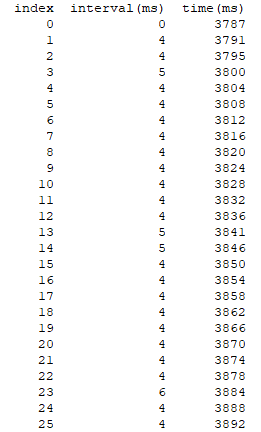
\includegraphics[height=8cm]{images/arduino_uno.png}
    \captionof{figure}{Capture d'écran des acquisitions réalisées via l'Arduino Uno avec un délai nul.}
\end{center}

Nous voulons cependant attirer l'attention du lecteur sur le fait que le code Arduino utilisé génère des données aléatoirement avant de les envoyer vers l'interface graphique. Le temps d'exécution peut donc différer des résultats obtenus ci-dessus lorsque les données envoyées sont celles qui correspondent aux différents capteurs du dispositif.

\subsection{Arduino Due}
A nouveau, on peut observer que l'exécution de la boucle principale prend 4 à 5 millisecondes. Il n'est donc pas possible, même avec une Arduino Due, d'acquérir de nouvelles données toutes les millisecondes.

\begin{center}
    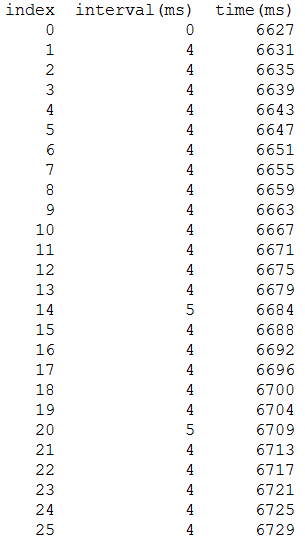
\includegraphics[height=8cm]{images/arduino_due.png}
    \captionof{figure}{Capture d'écran des acquisitions réalisées via l'Arduino Due avec un délai nul.}
\end{center}

Il semblerait donc que l'Arduino Due n'est pas plus puissante que l'Arduino Uno, et ne permet donc pas d'acquérir des données plus rapidement. Cependant, comme mentionné plus haut, les données utilisées pour réaliser ce test ont été générées aléatoirement par le code Arduino. Nous pensons qu'en opérant la même expérience mais avec les données mesurées par les différents capteurs, une différence de vitesse d'exécution plus marquée pourrait être observable. On peut en effet envisager l'hypothèse que l'Arduino Due soit plus puissante que l'Arduino Uno pour effectuer la conversion de la valeur expérimentale analogique en une valeur digitale.

\newpage
\section{Remarques supplémentaires}

\subsection{Remarques concernant le cahier des charges}
Au fur et à mesure de l'avancement du projet, l'utilité du bouton \textit{Recall} est devenue floue. Par conséquent, il a été décidé de ne pas l'implémenter.\\

La superposition de la force et de la position sur le même graphique ne constituant pas une fonctionnalité indispensable, il a été décidé de ne pas l'implémenter. Toutefois, le code actuel permet de rajouter cette fonction assez facilement: il suffirait de rajouter une boite à cocher dans le cadre dédié aux options de la force ("Force Options Frame" sur la figure \ref{fig:schemaDrawPlotsParent}). Lorsque cette boite est cochée, il faudrait créer un deuxième axe Y sur le graphique de la force (afin d'avoir une échelle différente) et y afficher les données de la position. L'implémentation de cette fonctionnalité nécessite, en plus de rajouter la boite à cocher, la modification de la méthode \textit{refresh\_all\_plots()} de \textit{DrawPlotsRealTime} et de \textit{DrawPlotsFromFile}.\\

Le but principal de l'acquisition en temps réel est d'afficher les données reçues sur les graphes. Cependant, il est apparu vers la fin du projet qu'il pourrait être nécessaire de stocker les données sur le microcontrôleur et de les envoyer vers l'interface lorsque l'acquisition est terminée. Il faut donc s'assurer que le code Python est adapté à cette contrainte ce qui semble être le cas lorsque l'on regarde la méthode \textit{real\_time\_data\_acquisition} de \textit{DrawPlotsRealTime}.

\subsection{Remarque concernant de possibles problèmes d'affichage de l'interface}

L'interface graphique peut ne pas s'afficher correctement sur tous les écrans (Comme présenté sur la figure \ref{fig:scale125}, certains éléments peuvent être hors des cadres et il est donc impossible d'interagir avec eux). Pour régler ce problème, deux méthodes existent:
\begin{enumerate}
    \item Modifier \textit{FIGURE\_X} et \textit{FIGURE\_Y} dans \textit{GlobalConfig}. Ceci va modifier la taille de la figure comprenant les 4 graphes ce qui peut permettre d'afficher tous les éléments si la figure est réduite.
    
    \item Changer la mise à l'échelle dans Windows ("Windows scaling"). La procédure est expliquée ci-dessous.
\end{enumerate}

Il faut commencer par faire un clique droit sur le bureau et choisir l'option "paramètres d'affichage" (display settings en anglais).
\begin{center}
    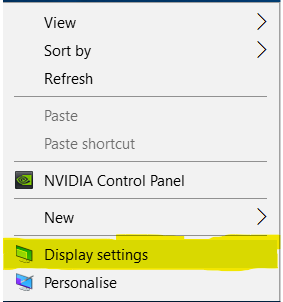
\includegraphics[scale=1]{images/windows_scaling_1.png}
    \captionof{figure}{Menu lorsqu'un clique droit est effectué sur le bureau}
\end{center}
    
On voit ci-dessous à gauche que la mise à l'échelle est de 125\%. La mise à l'échelle minimale est de 100\% et elle permet de maximiser le nombre d'éléments qui peuvent être affichés à l'écran.\\

\begin{center}

    % \begin{tabular}{cc}
    \begin{tabular}{p{8cm}p{8cm}}
        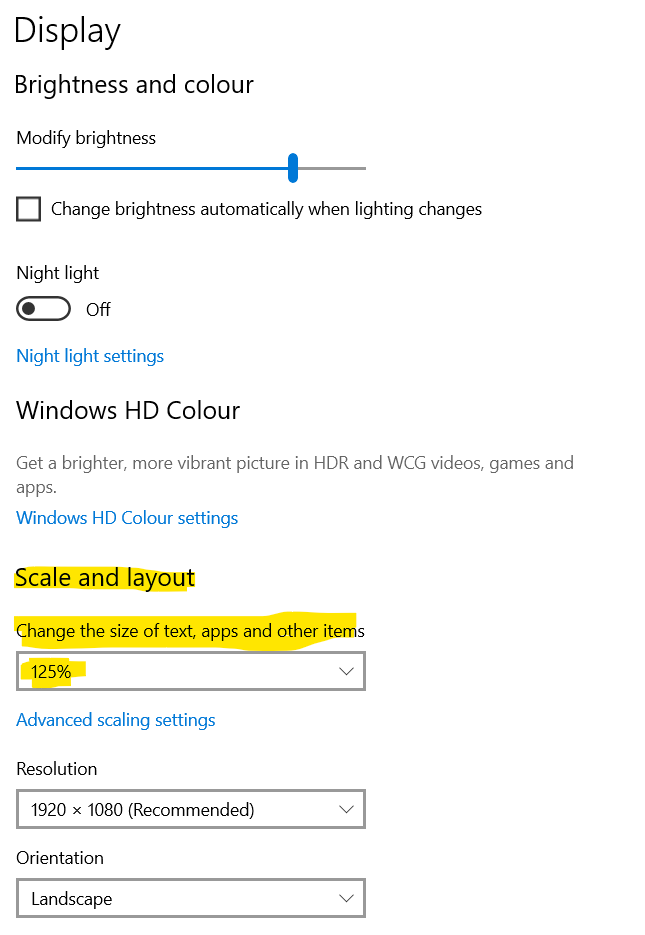
\includegraphics[height=10cm]{images/windows_scaling_2.png}
        \captionof{figure}{Mise à l'échelle: 125\%}
        &
        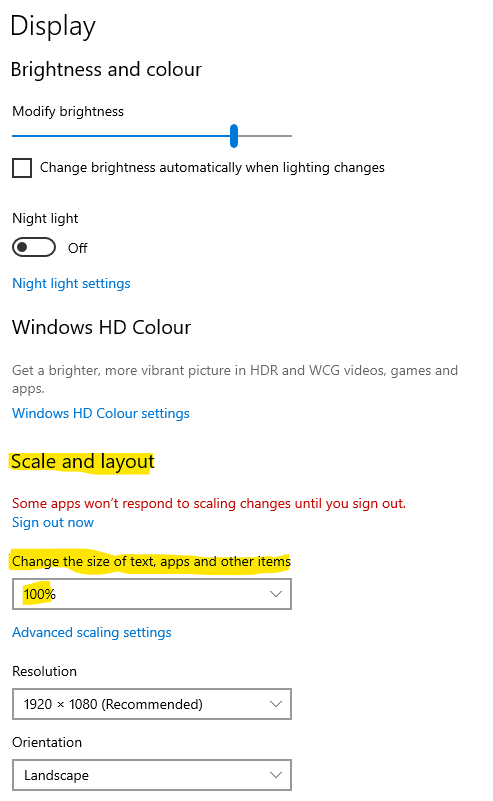
\includegraphics[height=10cm]{images/windows_scaling_3.png}
        \captionof{figure}{Mise à l'échelle: 100\%}
    \end{tabular}

\end{center}

Les deux images ci-dessous permettent de voir l'impact du changement de ce paramètre.

\begin{center}
    
    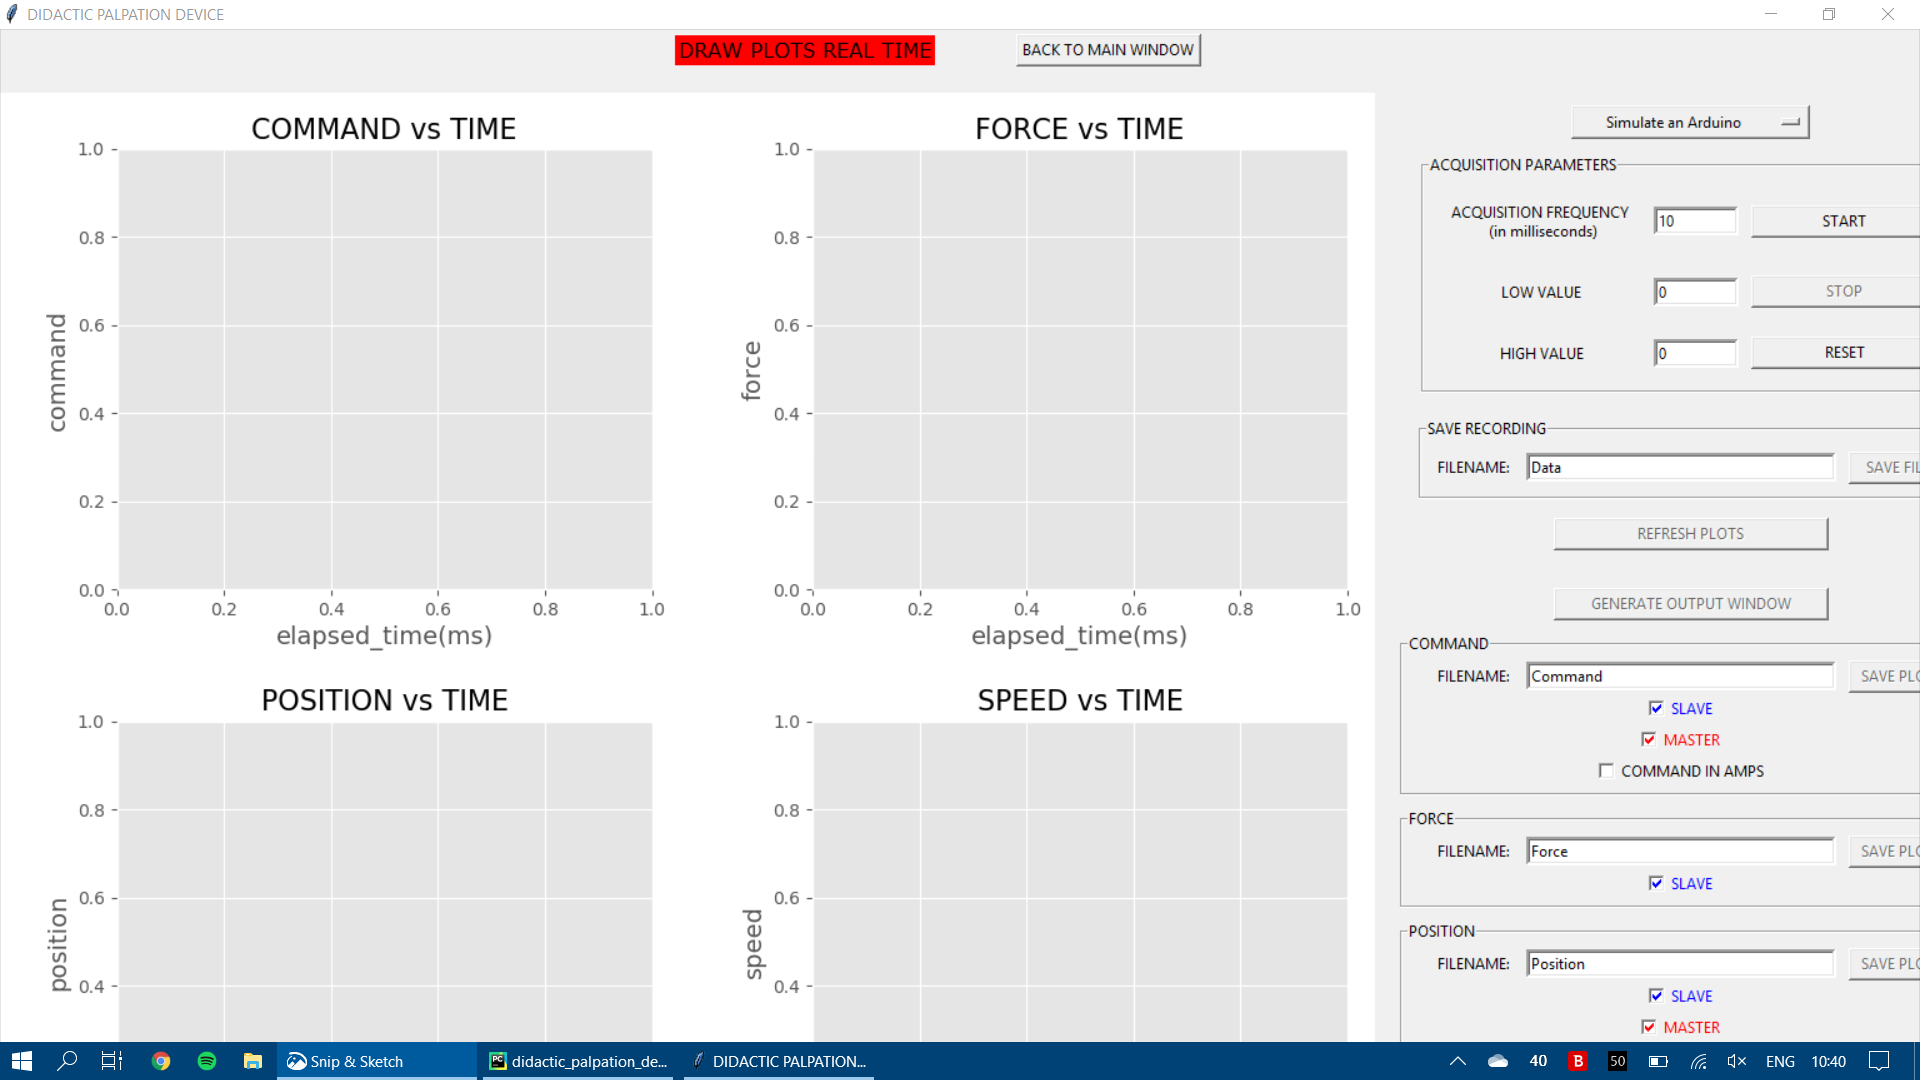
\includegraphics[width=17cm]{images/windows_scaling_4.png}
    \captionof{figure}{Mise à l'échelle: 125\%}
    \label{fig:scale125}
    
    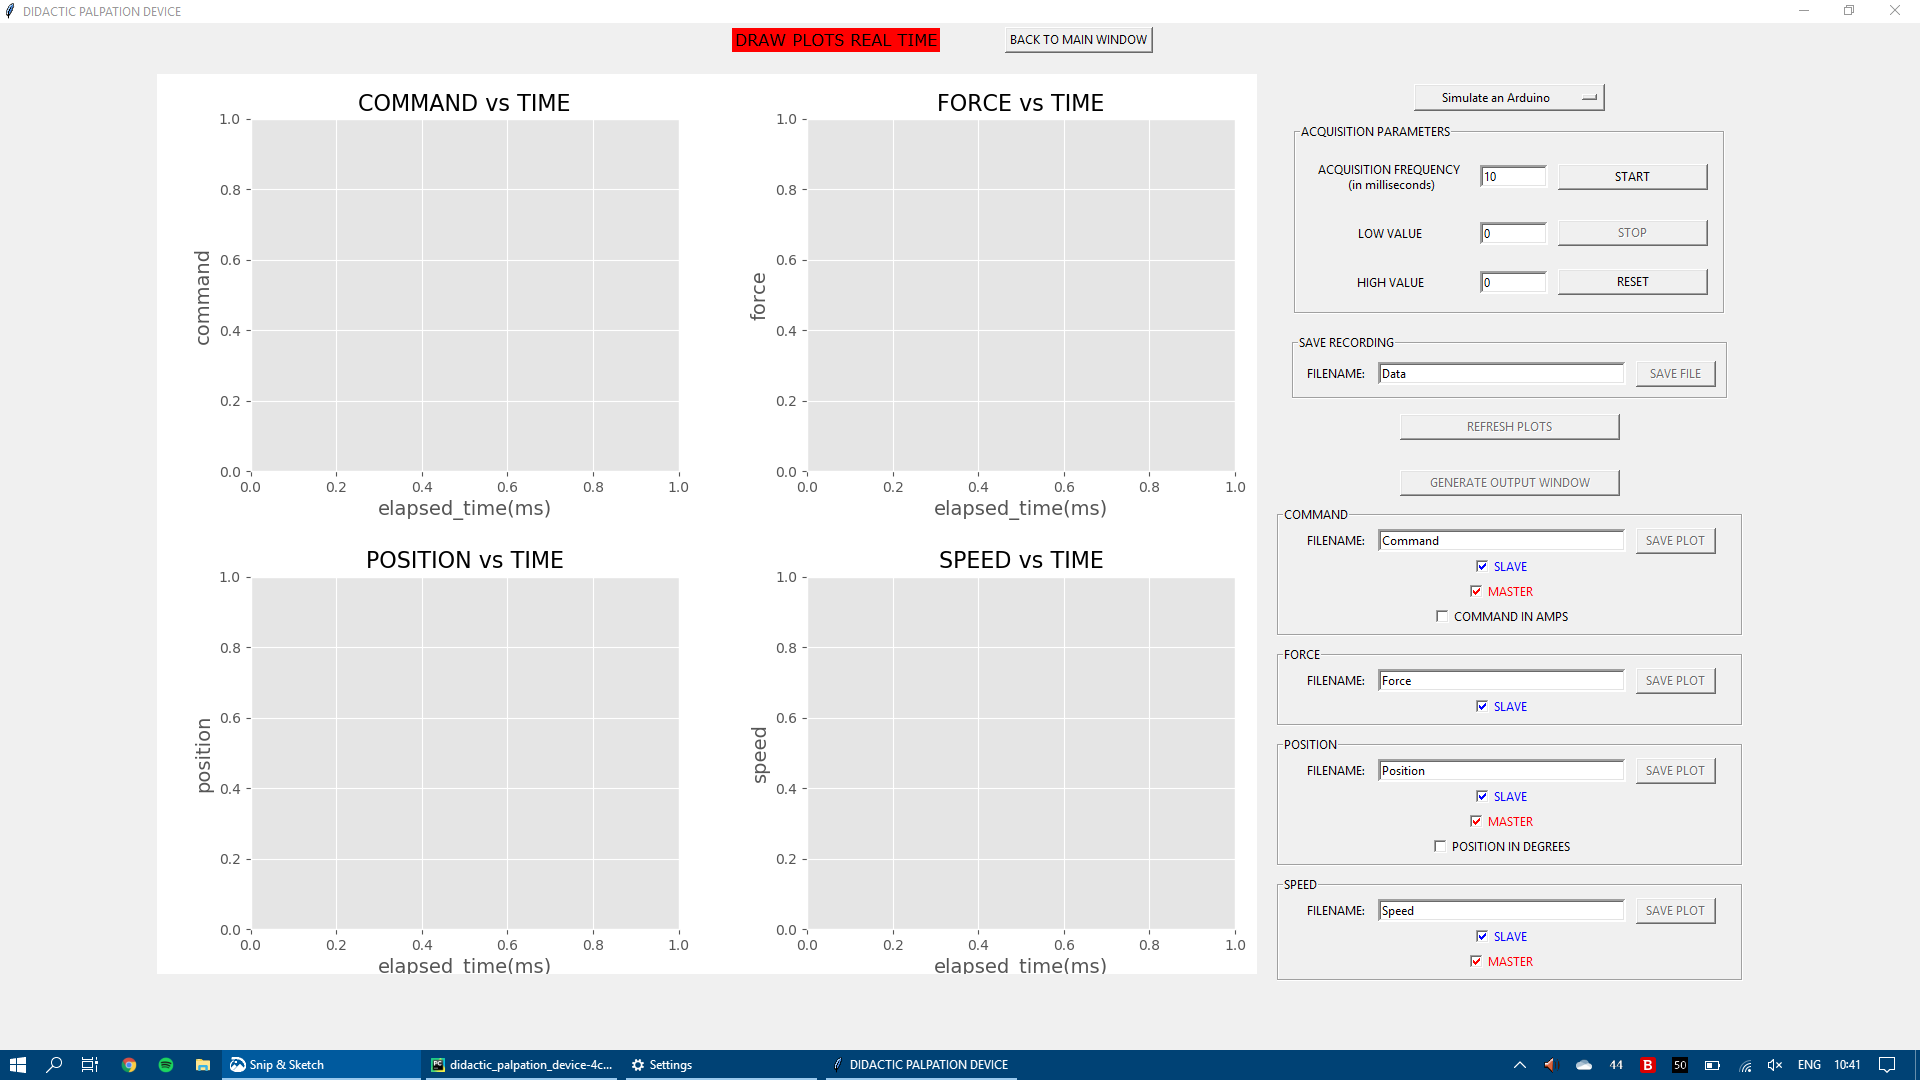
\includegraphics[width=17cm]{images/windows_scaling_5.png}
    \captionof{figure}{Mise à l'échelle: 100\%}

\end{center}

\newpage
\section{Développements futurs}

Pour conclure, nous proposons ci-dessous des recherches et vérifications complémentaires afin de s'assurer le bon fonctionnement de l'interface.

\begin{enumerate}
    \item Nous recommandons de s'assurer que le programme est utilisable sur toute taille/résolution d'écran et, le cas échéant, implémenter les changements nécéssaires. 
    
    \item Lorsque l'acquisition des données dure longtemps, les graphes deviennent illisibles. Il pourrait être intéressant de n'afficher que les 10 ou 20 dernières secondes de l'acquisition afin d'assurer une meilleure lisibilité.
    
    \item Investiguer s'il est en effet possible pour l'Arduino d'envoyer les données toutes les millisecondes grâce au code du microcontrôleur qui est spécifique au \textit{didactic palpation device}.
    
    \item Nous avons parfois observé des légères pertes de données lorsque l'acquisition dure longtemps. Ceci est typique d'un \textit{buffer} plein. Nous pensons que ce problème peut être lié au temps requis pour ajouter les données aux différentes listes. En effet, lorsqu'une liste est initialisée, elle est représentée sous forme de tableau de taille fixe (par exemple, de taille \textit{n}). Lorsque cette liste est pleine après le rajout de n éléments, l'ajout du \textit{n+1} élément nécessite de créer un nouveau tableau de taille \textit{2n}, d'y copier les \textit{n} éléments et d'y ajouter l'élément \textit{n+1}. Lorsque les tableaux deviennent grands, cette opération peut prendre plusieurs millisecondes\footnote{D'après nos tests. Le code pour afficher le temps requis pour l'opération est encore présent (voir \textit{real\_time\_data\_acquisition} dans \textit{DrawPlotsRealTime}} ce qui peut provoquer un embouteillage dans le \textit{buffer}. Il serait donc intéressant de faire des investigations complémentaires afin de s'assurer que le problème provient bien de cette opération et d'y trouver des solutions.\\
    
    
\end{enumerate}